\chapter{Evaluation}
\label{cap:cap05}

%*In this chapter we evaluate our work in terms of the requisites presented on section \ref{sec:sec02}. The first section shows in numbers how many features are covered by the software switch. Subsequently, in the next section, we present the results of performance benchmarks tests. The last section of the chapter is a qualitative evaluation about the code's ease to change. We demonstrate the code portability, highlighting the port of the software switch to another processor architecture in a different operating system.      

We propose two methods to evaluate our prototype: The first one focused in asses the functionality of the pipeline and controller, therefore, this evaluation will be present along BNG development with virtual interfaces, the second one is using our BNG software switch with MACSAD tool in a Linux server to run, compile and assess the performance in a real environment with 10G NIC. Details below:

\section{Functional Evaluation}
We assess the functionality of the control plane of the BNG software switch using a packet generator (Scapy) to generate and transmit packets through it and a network protocol analyzer (Wireshark) in a development environment to verify the sent and received packets along the virtual interfaces. The BNG functions to be evaluated are: 

\begin{itemize}
	\item Lookup tables
	\item L3 forwarding
	\item Mac learning
	\item Encap/Decap GRE header
	\item Network address translation
	\item Traffic manager 
	\item Controller functions like send entry tables
\end{itemize}

\section{Performance Evaluation}
\begin{itemize}
	\item It is important to judge the performance of  \acrshort{BNG} device, considering that we could have millions of packets trough it. 
	In order to validate the BNG software switch in a real network environment, we will compile on the Macsad tool in a commodity server, where the BNG software switch interfaces are connected to the Network Function Performance analyzer (NFPA \cite{nfpa}) node  via two 10G links to generates test traffic (See figure \ref{fig:bng_perf} ).
	
	
	\begin{figure}[ht]
		\centering
		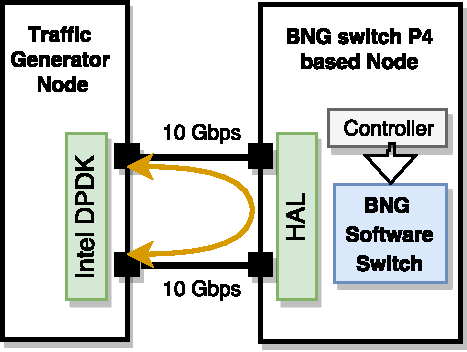
\includegraphics[width=0.35\linewidth] 
		{figures/bng_perf.pdf}
		\caption{BNG performance evaluation scenario.}
		\label{fig:bng_perf}
	\end{figure}
	
	This proof-of-concept implementation, will be run over Macsad server than will receive and forward the packets from Port 0 to Port 1, the NFPA node linked with MACSAD will send the packets and analyze the throughput in packets per second (pps) and bits per second (bps).\\
	
	For the BNG best-case test, the NFPA node will transmit packets with a fixed source and destination MAC addresses, and IP addresses, TCP port, and tunnel IP addresses, the configurations of the tables are presented,   in figure \ref{fig:bng_tables}
	For complex use case, the NFPA provides a wide selection of traffic traces with different packet headers and sizes,  for example with 1 to 1 million of packets with different flows and each one having different destination and source MAC addresses, different source and destination IP addresses, different TCP ports, different GRE IP addresses plus
	different source and destination port.
	
	\begin{figure}[ht]
		\centering
		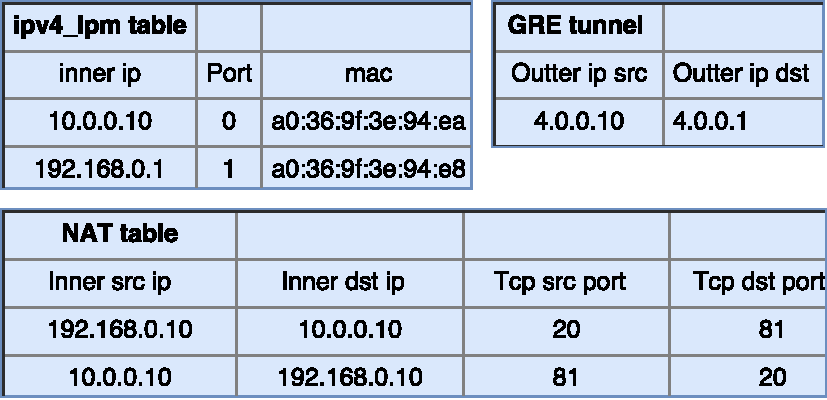
\includegraphics[width=0.6\linewidth] 
		{figures/bng_tables.pdf}
		\caption{Best-case Tables information.}
		\label{fig:bng_tables}
	\end{figure}
	
	
	
\end{itemize}




\subsection{Performance Benchmarks}

*One of the software switch requirements listed on chapter \ref{cap:intro} is to reach Line rate. For this reason we evaluated the switch performance in terms of network metrics. In this section we show how the switch performs for different packet sizes in comparison with other related BNG/BRAS implementation.   
The machine configuration used to perform measurement tests are listed in the box below. 

\begin{framed}

\begin{itemize}
\item \textbf{Processor}: Intel Xeon E5-2620v2 processors (6 cores, HT-disabled)
\item \textbf{Memory}:	64GB 
\item \textbf{Operating}: System	Ubuntu 16.04 (Kernel 4.4) LTS
\item \textbf{NIC}: dual-port Intel X540-AT2 (10G)

\end{itemize}

\end{framed}

    \subsubsection{Maximum Throughput}
    \label{sec:MaxBand}
    *This test evaluates the maximum forwarding rate the software switch can reach in comparison to other userspace implementations. 
    
    *The setup for maximum throughput evaluation is the following:
    
    \begin{itemize}
    \item A running instance of the BNG software switch with two Network interfaces cards - Port 1 and Port 2 - attached. 
    \item One set of tables entries installed in the Flow Table to match a packet sent to Port 1 with destiny ethernet 00:00:00:00:01. The action is an output packet to Port 2. 
    \item A packet traffic generator. We used a Open source program named NFPA.   
    \end{itemize}
    
    %The test starts by installing the flow in the switch Flow Table. Afterwards, we inject packets, using the traffic generator, directly into Port 1. The bandwidth results of Port 2, reported by the script, are used to calculate the average rate and the standard deviation.  
    %Two transmission measurements were made: for small packets of 64Kb and bigger packets of 1500Kb. Figure \ref{graph:comparison} shows results for both experiments.


  
   %Switch forwarding performance for small packets is evaluated in Kilo packets per second (Kpps). Figure \ref{graph:comparison64} shows that ofsoftswitch13 can handle 38.08 Kpps. This result is very 
   %far from Trema and approximatelly 32\% more efficient than LINC. Bigger packets are measured in Megabits per second. Results presented in Figure \ref{graph:comparison1500} show that ofsoftswitch13 and LINC, with rates of 260.25 Mbps 280.35 Mbps respectively, are slower than Trema with a bandwidth of 843.56 Mbps. 

    






